\chapter{Исследовательская часть}

\section{Технические характеристики}

Технические характеристики устройства, на котором выполнялись замеры времени, представлены далее:

\begin{itemize}
	\item процессор -- 2 Гц 4‑ядерный процессор Intel Core i5;
	\item оперативная память -- 16 ГБайт;
	\item операционная система -- macOS Venura 13.5.2. 
\end{itemize}

\section{Примеры работы программы}

На рисунке \ref{lst:LM} представлен пример работы программы.

\begin{lstlisting}[label=lst:LM,caption=Пример работы программы]
	ivanmamvriyskiy@h54 main % ./a.out 
    Меню:
    1)Одинчный подсчет;
    2)Замер времени;
    3)Выход.
    1
    Введите размерность матрицы N: 3
    1 2 3
    4 0 5
    6 7 0
    Обратная матрица: 
    -0.321101 0.192661 0.091743 
    0.275229 -0.165138 0.064220 
    0.256881 0.045872 -0.073394 
    Обратная матрица параллельным алгоритмом: 
    -0.321101 0.192661 0.091743 
    0.275229 -0.165138 0.064220 
    0.256881 0.045872 -0.073394 
\end{lstlisting}

\section{Время выполнения алгоритмов}

На рисунке \ref{img:graph}  представлена зависимость времени выполнения алгоритма от размерности матрицы при различных 
количествах потоков: последовательный алгоритм, 8 потоков (оптимальное количество), и 32 потока (для демонстрации затрат на
переключение ядер при превышении оптимального количества потоков). Таким образом, график показывает время работы программы с
и без распараллеливания.

\begin{table}[!ht]
    \centering
    \caption{\label{tab:table} Время выполнения работы алгоритмов в зависимости от размерности 
    матрицы и количества потокв(мс).}
    \begin{tabular}{|r|r|r|r|r|r|r|}
        \hline
            Размеренность & 1 & 2 & 4 & 8 & 16 & 32 \\ \hline
            1 000 & 13 & 7 & 4 & 3 & 3 & 4 \\ \hline
            2 000 & 57 & 31 & 15 & 13 & 13 & 13 \\ \hline
            3 000 & 127 & 65 & 48 & 55 & 56 & 61 \\ \hline
            4 000 & 264 & 140 & 111 & 92 & 100 & 103 \\ \hline
            5 000 & 434 & 245 & 182 & 162 & 164 & 166 \\ \hline
            6 000 & 636 & 367 & 268 & 240 & 243 & 244 \\ \hline
            7 000 & 948 & 610 & 411 & 356 & 358 & 370 \\ \hline
            8 000 & 1 347 & 769 & 618 & 443 & 480 & 496 \\ \hline
            9 000 & 1 516 & 930 & 687 & 553 & 607 & 732 \\ \hline
            10 000 & 1 710 & 1 093 & 741 & 698 & 816 & 878 \\ \hline
        \end{tabular}
\end{table}

\clearpage

\begin{figure}[h]
	\centering
	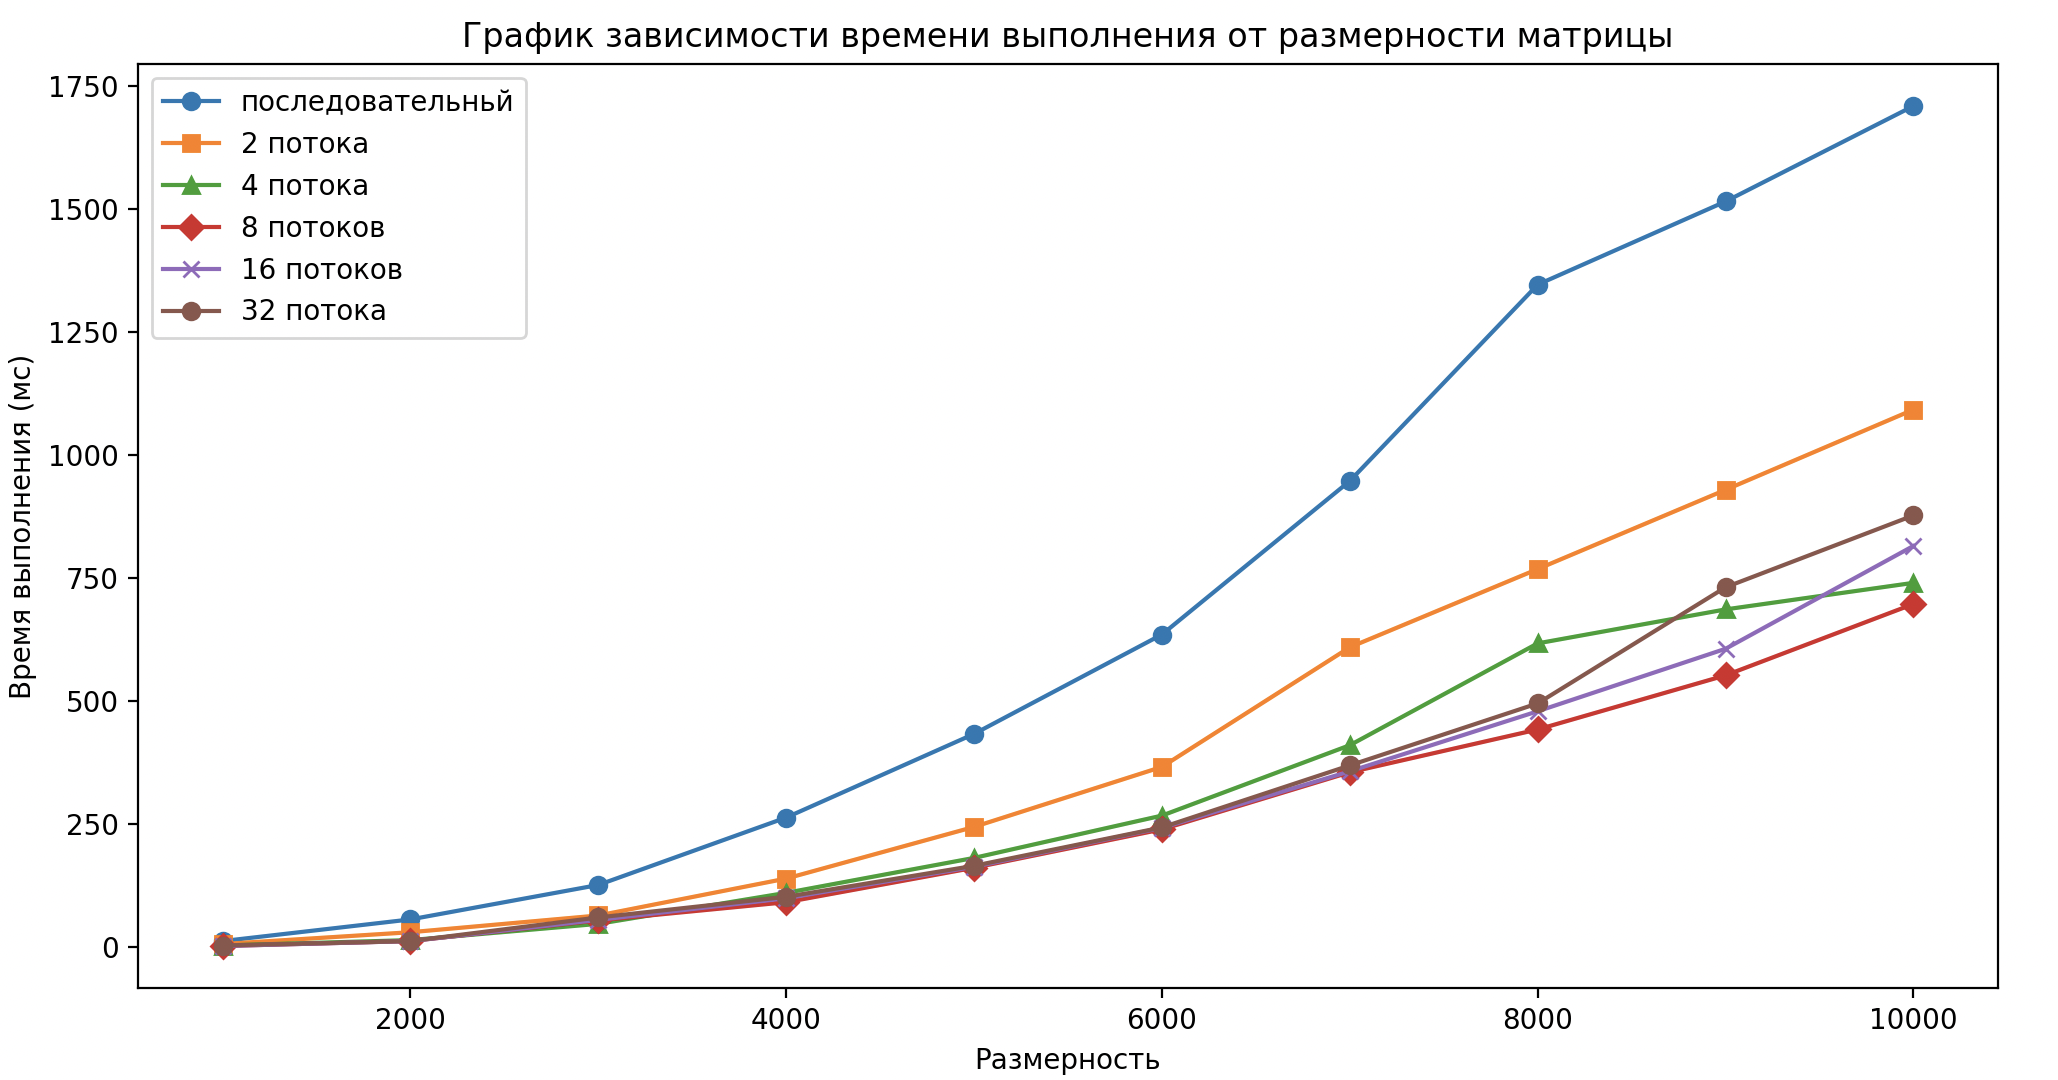
\includegraphics[width=1\textwidth]{img/graph.png}
	\caption{График зависимости времени выполнения работы от размерности матрицы при различных количествах потоков}
	\label{img:graph}
\end{figure}

По результатам замера времени можно сделать следующие выводы:
\begin{itemize}
	\item при движении от наименьшего числа потоков к числу логических ядер
	время работы алгоритма уменьшается;
    \item при превышении числа логических ядер время увеличивается, так как 
    затрачивается время на переключение ядра между потоками;
    \item последовательная реализация работает примерно в 3 раз медленне,
    чем реализация с использованием оптимального количества
    потоков, то есть 8 потоков.
\end{itemize}


\section{Вывод}

Таким образом, для максимального ускорения работы программы
с помощью распараллеливания необходимо использовать оптимальное число 
логических ядер. 
